\newpage

%   (III $\cup$ II)' $\cap$ (II' $\cap$ I)' 
\textbf{e)} Analizando paso por paso el segundo inciso \ref{e}, se puede resolver en dos partes \textbf{(III $\cup$ II)'} y \textbf{(II' $\cap$ I)' } para así unir ambos subconjuntos \\

Resolviendo \textbf{(III $\cup$ II)' }

\begin{align*}
(III \cup II)'   &= (\{ a, b, c, d, e, f, g, h, i, j, o, u  \}  \cup \{ h, j, p, q, r, s  \})' \\
  &=    (\{ a, b, c, d, e, f, g, h, i, j, o, p, q, r, s, u, \})'      \\
  &=   \{  k, l, m, n, t, v, w, x, y, z \}      \\
\end{align*}

Resolviendo \textbf{(II' $\cap$ I)' }

\begin{align*}
(II' \cap I)'   &= ( \{ a, b, c, d, e, f, g, i, k, l, m, n, o, t, u, v, w, x, y, z \} \cap \{a, e, i, o, u\} )' \\
  &=    (\{a, e, i, o, u\})'      \\
  &=  \{ b, c, d, f, g, h, j, k, l, m, n, p, q, r, s, t, v, w, x, y, z \}      \\
\end{align*}

Juntando ambos lados para armar (III $\cup$ II)' $\cap$ (II' $\cap$ I)':

\begin{align*}
(III \cup II)' \cap (II' \cap I)'  &= \{  k, l, m, n, t, v, w, x, y, z \} \cap \{ b, c, d, f, g, h, j, k, l, m, n, p, q, r, s, t, v, w, x, y, z \}  \\
  &= \{ k, l, m, n, t,  v, w, x, y, z \}
\end{align*}

Por lo tanto el resultado es:

\begin{equation*}
    \boxed{(III \cup II)' \cap (II' \cap I)'  =   \{ k, l, m, n, t,  v, w, x, y, z \}   }
\end{equation*}



Para obtener el diagrama de Venn, se puede hacer por partes, el lado derecho y lado izquierdo, quedando: \\

\textbf{(III $\cup$ II)'}: 

\begin{figure}[htbp]
\centering
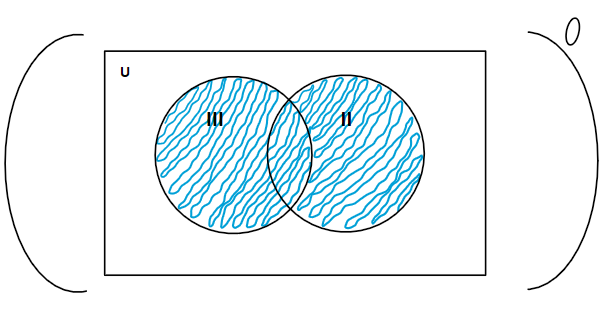
\includegraphics[width=8cm]{e/aa.png}
\caption[]{Diagrama de Venn de (III $\cup$ II)'}
\end{figure} 

\newpage

Sacando el complemento, queda el diagrama

\begin{figure}[htbp]
\centering
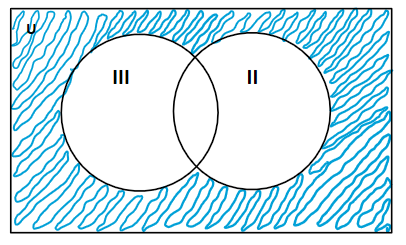
\includegraphics[width=8cm]{e/aaa.png}
\caption[]{Diagrama de Venn de (III $\cup$ II)'}
\end{figure} 

\textbf{(II' $\cap$ I)'}:

\begin{figure}[htbp]
\centering
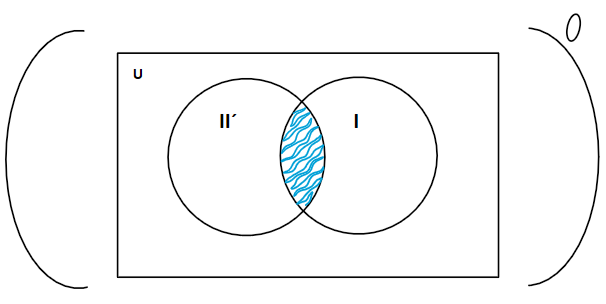
\includegraphics[width=8cm]{e/bb.png}
\caption[]{Diagrama de Venn de (II' $\cap$ I)'}
\end{figure} 

Sacando el complemento, queda el diagrama

\begin{figure}[htbp]
\centering
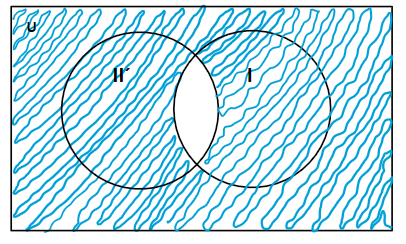
\includegraphics[width=7cm]{e/bbb.png}
\caption[]{Diagrama de Venn de (II' $\cap$ I)'}
\end{figure} 


\newpage

Haciendo la intersección de ambos lados para armar (III $\cup$ II)' $\cap$ (II' $\cap$ I)' , quedando así el diagrama de Venn:

\begin{figure}[htbp]
\centering
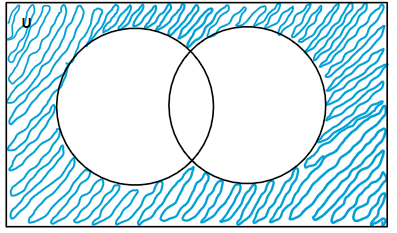
\includegraphics[width=8cm]{e/aabb.png}
\caption[]{Diagrama de Venn de (III $\cup$ II)' $\cap$ (II' $\cap$ I)' }
\end{figure} 
